\section{Sistemi operativi e freeRTOS}
I uC normalmente non hanno dei sistemi operativi o meglio, ogni uC potrebbe avere il proprio pensato e scritto dalla azienda che lo produce.
Tra quelli più conosciuti e pubblicizzati ci sono:
\begin{itemize}
    \item freeRTOS: completamente gratuito e la licenza permette gli utilizzi commerciali.
    \item Chibios
\end{itemize}

Per l' ATmega32 non è disponibile freeRTOS ma è semplice portarlo in quanto esiste già per ATmega328.
Per portarlo da una architettura all' altra bisogna cambiare alcune impostazioni in base all' architettura ed alle periferiche che il uC monta.

Ognuno di questi sistemi operativi utilizza ovviamente della RAM e tiene un timer in utilizzo solo per lui.

L' utilizzo principale è quello di spezzare un problema difficile in tanti problemi piccoli, ogni problema viene gestito in un singolo processo.

\subsection{Funzionamento di un sistema operativo generico}
In memoria da qualche parte si trova il codice del sistema operativo, questo è il primo codice che viene eseguito.
Dopo che il sistema operativo ha eseguito delle inizializzazioni per far funzionare il sistema appieno si lascia il comando al primo processo detto \verb{init{.
Questo primo processo successivamente può crearne altri utilizzando la primitiva del sistema operativo \verb{fork{, questa funzione crea ua copia 1:1 del processo corrente, il nuovo processo poi può cambiare il suo codice caricandone un altro usando la primitiva \verb{exec{.
Così facendo ogni processo può crearne altri e diversi.
Questo è anche il comportamento di una shell tipica del terminale.

\subsubsection{Kernel e processi}
Dopo che il sistema operativo ha dato il controllo al primo processo, il processore prenderà ad eseguire esclusivamente processi.
Il kernel torna ad essere eseguito solo se:
\begin{itemize}
    \item un processo richiede dei servizi al kernel (aprire un file, fork, exec, ecc, ecc)
    \item arrivano delle interruzioni che devono essere gestite dal kernel
\end{itemize}

Il kernel non è quindi un processo vero e proprio e non termina mai.

\subsection{freeRTOS}
Essendo un sistema operativo pensato per i microcontrollori, spesso non fa uso della MMU (in quanto potrebbe non esserci).
Si fa quindi il linking di tutti i processi e dello stesso kernel assieme e tutte queste parti sono caricati nella stessa mappa di memoria.

Per chiedere al sistema operativo alcuni servizi si usano delle semplici chiamate a funzioni in quanto non c'è un cambio di privilegi per passare da processo utente a kernel.

\subsubsection{Processi}
L' elenco dei processi si trova nella struttura dati TCB: Task Control Block che è un array di strutture dati utili per l' evoluzione dei processi.
Alcune funzioni possono essere in comune tra più processi quindi la mappa di memoria non per forza è una sequenza di processi diversi, potremo avere invece processi spezzettati in diverse aree di memoria.

Abbiamo una unica sezione \verb{.bss{ ed una unica sezione \verb{.data{, tutti i dati sono quindi pubblici.
Di privato invece c'è lo stack quindi se un processo dichiara le proprie variabili sullo stack esse saranno private, quando si cambia processo in esecuzione quindi va cambiato lo stack.

\subsubsection{Cambio di processo}
Quando un processo chiama il kernel per un servizio il kernel controlla le precedenze dei processi e mette in esecuzione quello più urgente.
Quindi il kernel non è detto che rimetta in esecuzione il processo che lo ha chiamato.
Questo cambio di processo può accadere anche quando arriva una interruzione, che viene quindi gestita dal kernel e successivamente sceglie un processo da mettere in esecuzione.

Quando si ha un cambio di processo è necessario salvare i registri del processo corrente e mettere quelli del processo nuovo, questi valori vengono salvati nello stack tramite varie push, invece SP viene salvato nel TCB.

Si ha quindi una illusione di multitasking tra questi processi in quanto ho vari processi che vengono eseguiti un po' ciascuno.

Il cambio di processo tuttavia è molto dispendioso proprio per questo salvataggio dei registri.

I processi in freeRTOS hanno priorità statica fissata a tempo di compilazione quindi quando si deve scegliere quale processo mettere in esecuzione si guarda a quello con priorità minore.
In caso di parità si fa a turni in modo da farli evolvere tutti.

\subsubsection{Stati di un processo}
Un processo può trovarsi in uno di questi 3 stati:
\begin{figure}[H]
    \centering
    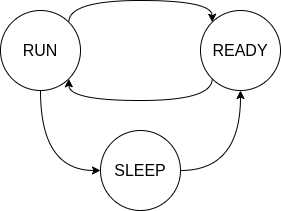
\includegraphics[width=150px]{images/30_freeRTOS/task_evolution.png}
\end{figure}
Un processo è in sleep se si trova in attesa di qualcosa, questo comportamento è ottimale per evitare attese attive, quando devo fare qualcosa che potrebbe portarmi ad aspettare la inizio e poi mi metto in pausa fino all' arrivo di una interruzione che mi segnali la fine.

Posso anche chiedere di andare in sleep per un tot di tempo, anche qui è comodo per evitare di buttare tempo CPU utile.

\subsubsection{Esempio su ATmega328}
\begin{verbatim}
    void main(){
        atmel_start_init();
            // Si usa per inizializzare le periferiche
            // di questo processore
            
        VStartRegTestTasks();
            // Lancia un task standard
        
        
        xTaskCreate(funzione_task,  // puntatore a funzione
                "nome_task",        // stringa nome del processo
                23,                 // dimensione dello stack
                NULL,               // puntatore ai parametri
                5,                  // priorità
                NULL);              // 
    
        vTaskStartScheduler();
            // Fa partire lo scheduler e sceglie
            // quale processo mettere in esecuzione
            // Avvia anche l' idle task, cioè il processo
            // a priorità minima da mettere in esecuzione
            // se non c'è niente da fare
    }
\end{verbatim}

\subsection{Sincronizzazione}
Se ci sono alcune periferiche che devono essere usate da più processi oppure c'è bisogno di scambiarsi dei dati tra processi queste rihieste e questi messaggi vengono messi in alcune liste.
Le liste sono di dimensione fissa quindi una volta riempita tutta al prossimo inserimento il processo viene stoppato e messo in coda sleep.

Per effettuare queste operazioni si usano delle primitive di sincronizzazione come i semafori.

\subsubsection{Sezione critica}
Possiamo creare una sezione critica disabilitando le interruzioni e l' azione dello scheduler utilizzando le primitive:
\begin{itemize}
    \item \verb{vTaskSuspendAll{: sospende lo scheduler e disabilita le interruzioni
    \item \verb{xTaskResumeAll{: riabilita lo scheduler e le interruzioni
\end{itemize}
tra la prima chiamata e la seconda chiamata il processo non può essere stoppato. 

